\chapter{Results}
\label{sec:appendix-b}
This appendix contains the remaining demographic analysis of the survey results from section \ref{sec:results-demographics} and the experiments with the value-sensitive rejector from section \ref{sec:results-rejector}.

\section{Demographic analysis}
This section contains some additional tables about the demographic analysis.
%
Table \ref{tab:results-differences-grp} shows the group differences for the aggregated scenario types (TP, TN, FP, FN, and REJ).
%
Tables \ref{tab:results-pairwise-nationality}, \ref{tab:results-pairwise-language}, and \ref{tab:results-pairwise-ethnicity} show the pairwise group differences for the nationality, language, and ethnicity features, respectively.

\begin{table}[H]
    \small
    \centering
    \begin{tabular}{lccc|ccc}
        \toprule
                     & \multicolumn{3}{c}{\textbf{Two groups}} & \multicolumn{3}{c}{\textbf{More than two groups}}                                                                                                                                                                       \\
        \midrule
                     & \multicolumn{1}{c}{\textbf{Sex}}        & \multicolumn{1}{c}{\textbf{Student}}              & \multicolumn{1}{c}{\textbf{Continent}} & \multicolumn{1}{c}{\textbf{Nationality}} & \multicolumn{1}{c}{\textbf{Language}}  & \multicolumn{1}{c}{\textbf{Ethnicity}} \\
        \midrule
        \textbf{TP}  & 0.302                                   & \cellcolor[HTML]{EFEFEF}\textbf{0.032}            & 0.286                                  & 0.218                                    & 0.109                                  & 0.242                                  \\
        \textbf{TN}  & 0.726                                   & 0.379                                             & 0.204                                  & 0.190                                    & 0.216                                  & 0.281                                  \\
        \textbf{FP}  & 0.699                                   & 0.933                                             & 0.073                                  & \cellcolor[HTML]{EFEFEF}\textbf{0.020}   & \cellcolor[HTML]{EFEFEF}\textbf{0.040} & \cellcolor[HTML]{EFEFEF}\textbf{0.037} \\
        \textbf{FN}  & 0.961                                   & 0.150                                             & 0.847                                  & 0.478                                    & 0.438                                  & 0.584                                  \\
        \textbf{REJ} & 0.835                                   & 0.625                                             & 0.496                                  & 0.271                                    & 0.103                                  & 0.068                                  \\
        \bottomrule
    \end{tabular}
    \caption{\textbf{Aggregated}: an overview of the statistical differences between different groups of participants for various demographic characteristics for each aggregated scenario type in the ME survey. Each cell contains the p value of either the Mann-Whitney U test for two groups or the Kruskal-Wallis test for more than two groups. The grey cells with bold text indicate significant statistical differences between the groups for that feature and scenario type.}
    \label{tab:results-differences-grp}
\end{table}

\begin{table}[H]
    \scriptsize
    \centering
    \setlength\tabcolsep{2pt}
    \begin{subtable}{.44\textwidth}
        \centering
        \begin{tabular}{lcccc}
            \toprule
                                  & \textbf{South Africa} & \textbf{Poland}                        & \textbf{Portugal} & \textbf{Spain} \\
            \midrule
            \textbf{South Africa} & 1.000                 &                                        &                   &                \\
            \textbf{Poland}       & 0.077                 & 1.000                                  &                   &                \\
            \textbf{Portugal}     & 0.077                 & \cellcolor[HTML]{EFEFEF}\textbf{0.009} & 1.000             &                \\
            \textbf{Spain}        & 0.119                 & 0.083                                  & 0.613             & 1.000          \\
            \bottomrule
        \end{tabular}
        \caption{TP6}
    \end{subtable}%
    \begin{subtable}{.44\textwidth}
        \centering
        \begin{tabular}{cccc}
            \toprule
            \textbf{South Africa}                  & \textbf{Poland}                        & \textbf{Portugal}                      & \textbf{Spain} \\
            \midrule
            1.000                                  &                                        &                                        &                \\
            0.755                                  & 1.000                                  &                                        &                \\
            0.261                                  & 0.261                                  & 1.000                                  &                \\
            \cellcolor[HTML]{EFEFEF}\textbf{0.026} & \cellcolor[HTML]{EFEFEF}\textbf{0.038} & \cellcolor[HTML]{EFEFEF}\textbf{0.050} & 1.000          \\
            \bottomrule
        \end{tabular}
        \caption{FP2}
    \end{subtable}
    \vskip\baselineskip
    \begin{subtable}{.44\textwidth}
        \centering
        \begin{tabular}{lcccc}
            \toprule
                                  & \textbf{South Africa}                  & \textbf{Poland} & \textbf{Portugal} & \textbf{Spain} \\
            \midrule
            \textbf{South Africa} & 1.000                                  &                 &                   &                \\
            \textbf{Poland}       & 0.342                                  & 1.000           &                   &                \\
            \textbf{Portugal}     & 0.304                                  & 1.000           & 1.000             &                \\
            \textbf{Spain}        & \cellcolor[HTML]{EFEFEF}\textbf{0.043} & 0.304           & 0.220             & 1.000          \\
            \bottomrule
        \end{tabular}
        \caption{FP7}
    \end{subtable}%
    \begin{subtable}{.44\textwidth}
        \centering
        \begin{tabular}{cccc}
            \toprule
            \textbf{South Africa}                  & \textbf{Poland}                        & \textbf{Portugal} & \textbf{Spain} \\
            \midrule
            1.000                                  &                                        &                   &                \\
            \cellcolor[HTML]{EFEFEF}\textbf{0.034} & 1.000                                  &                   &                \\
            0.150                                  & \cellcolor[HTML]{EFEFEF}\textbf{0.011} & 1.000             &                \\
            \cellcolor[HTML]{EFEFEF}\textbf{0.045} & \cellcolor[HTML]{EFEFEF}\textbf{0.011} & 0.679             & 1.000          \\
            \bottomrule
        \end{tabular}
        \caption{FN5}
    \end{subtable}
    \vskip\baselineskip
    \begin{subtable}{.44\textwidth}
        \centering
        \begin{tabular}{lcccc}
            \toprule
                                  & \textbf{South Africa} & \textbf{Poland} & \textbf{Portugal} & \textbf{Spain} \\
            \midrule
            \textbf{South Africa} & 1.000                 &                 &                   &                \\
            \textbf{Poland}       & 0.095                 & 1.000           &                   &                \\
            \textbf{Portugal}     & 0.622                 & 0.095           & 1.000             &                \\
            \textbf{Spain}        & 0.104                 & 0.095           & 0.104             & 1.000          \\
            \bottomrule
        \end{tabular}
        \caption{FN6}
    \end{subtable} %
    \begin{subtable}{.44\textwidth}
        \centering
        \begin{tabular}{cccc}
            \toprule
            \textbf{South Africa} & \textbf{Poland} & \textbf{Portugal} & \textbf{Spain} \\
            \midrule
            1.000                 &                 &                   &                \\
            0.088                 & 1.000           &                   &                \\
            0.227                 & 0.088           & 1.000             &                \\
            1.000                 & 0.227           & 0.388             & 1.000          \\
            \bottomrule
        \end{tabular}
        \caption{REJ1}
    \end{subtable}%
    \vskip\baselineskip
    \begin{subtable}{.44\textwidth}
        \centering
        \begin{tabular}{lcccc}
            \toprule
                                  & \textbf{South Africa} & \textbf{Poland} & \textbf{Portugal} & \textbf{Spanish} \\
            \midrule
            \textbf{South Africa} & 1.000                 &                 &                   &                  \\
            \textbf{Poland}       & 0.098                 & 1.000           &                   &                  \\
            \textbf{Portugal}     & 0.098                 & 1.000           & 1.000             &                  \\
            \textbf{Spain}        & 0.098                 & 0.422           & 0.422             & 1.000            \\
            \bottomrule
        \end{tabular}
        \caption{REJ4}
    \end{subtable}
    \caption{\textbf{Nationality}: an overview of all pairwise Mann-Whitney U tests between the different nationalities for all scenarios where we found significant differences between all nationalities using the Kruskal-Wallis test. Each cell contains the p value of the Mann-Whitney U test between two groups of different nationalities. We corrected all p values with the Benjamini-Hochberg procedure. The grey cells with bold text indicate significant statistical differences between the two nationalities.}
    \label{tab:results-pairwise-nationality}
\end{table}

\begin{table}[H]
    \scriptsize
    \centering
    \setlength\tabcolsep{2pt}
    \begin{subtable}{.405\textwidth}
        \centering
        \begin{tabular}{lcccc}
            \toprule
                               & \textbf{English} & \textbf{Polish} & \textbf{Portugese} & \textbf{Spanish} \\
            \midrule
            \textbf{English}   & 1.000            &                 &                    &                  \\
            \textbf{Polish}    & 0.561            & 1.000           &                    &                  \\
            \textbf{Portugese} & 0.352            & 0.283           & 1.000              &                  \\
            \textbf{Spanish}   & 0.176            & 0.258           & 0.142              & 1.000            \\
            \bottomrule
        \end{tabular}
        \caption{TP3}
    \end{subtable}%
    \begin{subtable}{.405\textwidth}
        \centering
        \begin{tabular}{cccc}
            \toprule
            \multicolumn{1}{c}{\textbf{English}} & \multicolumn{1}{c}{\textbf{Polish}}    & \textbf{Portugese} & \textbf{Spanish} \\
            \midrule
            1.000                                & \multicolumn{1}{c}{}                   &                    &                  \\
            0.089                                & 1.000                                  &                    &                  \\
            0.119                                & \cellcolor[HTML]{EFEFEF}\textbf{0.007} & 1.000              &                  \\
            0.522                                & 0.089                                  & 1.000              & 1.000            \\
            \bottomrule
        \end{tabular}
        \caption{TP6}
    \end{subtable}
    \vskip\baselineskip
    \begin{subtable}{.405\textwidth}
        \centering
        \begin{tabular}{lcccc}
            \toprule
                               & \textbf{English}                       & \textbf{Polish} & \textbf{Portugese} & \textbf{Spanish} \\
            \midrule
            \textbf{English}   & 1.000                                  &                 &                    &                  \\
            \textbf{Polish}    & 0.321                                  & 1.000           &                    &                  \\
            \textbf{Portugese} & 0.321                                  & 1.000           & 1.000              &                  \\
            \textbf{Spanish}   & \cellcolor[HTML]{EFEFEF}\textbf{0.019} & 0.444           & 0.321              & 1.000            \\
            \bottomrule
        \end{tabular}
        \caption{FP7}
    \end{subtable}%
    \begin{subtable}{.405\textwidth}
        \centering
        \begin{tabular}{cccc}
            \toprule
            \textbf{English} & \textbf{Polish}                        & \textbf{Portugese} & \textbf{Spanish} \\
            \midrule
            1.000            &                                        &                    &                  \\
            0.070            & 1.000                                  &                    &                  \\
            0.209            & \cellcolor[HTML]{EFEFEF}\textbf{0.011} & 1.000              &                  \\
            0.647            & 0.164                                  & 0.838              & 1.000            \\
            \bottomrule
        \end{tabular}
        \caption{FN5}
    \end{subtable}
    \vskip\baselineskip
    \begin{subtable}{.405\textwidth}
        \centering
        \begin{tabular}{lcccc}
            \toprule
                               & \textbf{English}                       & \textbf{Polish} & \textbf{Portugese} & \textbf{Spanish} \\
            \midrule
            \textbf{English}   & 1.000                                  &                 &                    &                  \\
            \textbf{Polish}    & 0.895                                  & 1.000           &                    &                  \\
            \textbf{Portugese} & 0.439                                  & 0.721           & 1.000              &                  \\
            \textbf{Spanish}   & \cellcolor[HTML]{EFEFEF}\textbf{0.049} & 0.309           & 0.548              & 1.000            \\
            \bottomrule
        \end{tabular}
        \caption{FN7}
    \end{subtable}%
    \begin{subtable}{.405\textwidth}
        \centering
        \begin{tabular}{cccc}
            \toprule
            \textbf{English} & \textbf{Polish} & \textbf{Portugese} & \textbf{Spanish} \\
            \midrule
            1.000            &                 &                    &                  \\
            0.076            & 1.000           &                    &                  \\
            0.387            & 0.076           & 1.000              &                  \\
            0.149            & 0.711           & 0.096              & 1.000            \\
            \bottomrule
        \end{tabular}
        \caption{REJ1}
    \end{subtable}
    \vskip\baselineskip
    \begin{subtable}{.405\textwidth}
        \centering
        \begin{tabular}{lcccc}
            \toprule
                               & \textbf{English} & \textbf{Polish} & \textbf{Portugese} & \textbf{Spanish} \\
            \midrule
            \textbf{English}   & 1.000            &                 &                    &                  \\
            \textbf{Polish}    & 0.063            & 1.000           &                    &                  \\
            \textbf{Portugese} & 0.063            & 1.000           & 1.000              &                  \\
            \textbf{Spanish}   & 0.599            & 1.000           & 1.000              & 1.000            \\
            \bottomrule
        \end{tabular}
        \caption{REJ4}
    \end{subtable}%
    \begin{subtable}{.405\textwidth}
        \centering
        \begin{tabular}{cccc}
            \toprule
            \textbf{English} & \textbf{Polish} & \textbf{Portugese} & \textbf{Spanish} \\
            \midrule
            1.000            &                 &                    &                  \\
            1.000            & 1.000           &                    &                  \\
            0.489            & 0.452           & 1.000              &                  \\
            0.105            & 0.152           & 0.105              & 1.000            \\
            \bottomrule
        \end{tabular}
        \caption{REJ5}
    \end{subtable}
    \caption{\textbf{Language}: an overview of all pairwise Mann-Whitney U tests between the different spoken languages for all scenarios where we found significant differences between all spoken languages using the Kruskal-Wallis test. Each cell contains the p value of the Mann-Whitney U test between two groups of languages. We corrected all p values with the Benjamini-Hochberg procedure. The grey cells with bold text indicate significant statistical differences between the two languages.}
    \label{tab:results-pairwise-language}
\end{table}

\begin{table}[H]
    \scriptsize
    \centering
    \setlength\tabcolsep{2pt}
    \begin{subtable}{.275\textwidth}
        \centering
        \begin{tabular}{lccc}
            \toprule
                           & \textbf{White}                         & \textbf{Mixed}                         & \textbf{Black} \\
            \midrule
            \textbf{White} & 1.000                                  &                                        &                \\
            \textbf{Mixed} & 0.552                                  & 1.000                                  &                \\
            \textbf{Black} & \cellcolor[HTML]{EFEFEF}\textbf{0.028} & \cellcolor[HTML]{EFEFEF}\textbf{0.028} & 1.000          \\
            \bottomrule
        \end{tabular}
        \caption{FP7}
    \end{subtable}%
    \begin{subtable}{.21\textwidth}
        \centering
        \begin{tabular}{ccc}
            \toprule
            \multicolumn{1}{l}{\textbf{White}}     & \textbf{Mixed}                                             & \textbf{Black}            \\
            \midrule
            1.000                                  &                                                            &                           \\
            0.776                                  & \multicolumn{1}{r}{1.000}                                  &                           \\
            \cellcolor[HTML]{EFEFEF}\textbf{0.002} & \multicolumn{1}{r}{\cellcolor[HTML]{EFEFEF}\textbf{0.776}} & \multicolumn{1}{r}{1.000} \\
            \bottomrule
        \end{tabular}
        \caption{REJ4}
    \end{subtable}%
    \begin{subtable}{.21\textwidth}
        \centering
        \begin{tabular}{ccc}
            \toprule
            \multicolumn{1}{l}{\textbf{White}}     & \textbf{Mixed}            & \textbf{Black}            \\
            \midrule
            1.000                                  &                           &                           \\
            \cellcolor[HTML]{EFEFEF}\textbf{0.016} & \multicolumn{1}{r}{1.000} &                           \\
            1.000                                  & \multicolumn{1}{r}{0.112} & \multicolumn{1}{r}{1.000} \\
            \bottomrule
        \end{tabular}
        \caption{REJ7}
    \end{subtable}
    \caption{\textbf{Ethnicity}: an overview of all pairwise Mann-Whitney U tests between the different ethnicities for all scenarios where we found significant differences between all ethnicities using the Kruskal-Wallis test. Each cell contains the p value of the Mann-Whitney U test between two groups of ethnicities. We corrected all p values with the Benjamini-Hochberg procedure. The grey cells with bold text indicate significant statistical differences between the two ethnicities.}
    \label{tab:results-pairwise-ethnicity}
\end{table}

\section{Probability Density Functions}
This section contains the Probability density functions of the predictions of all models to both the \emph{seen} (figure \ref{fig:pdfs-seen}) and the \emph{unseen} (figure \ref{fig:pdfs-unseen}) datasets.
%
They help us understand the value-sensitive metric results in figures \ref{fig:metric-plots-all-values} and \ref{fig:metric-plots-tptn0}.

\begin{figure}[H]
    \centering
    \begin{subfigure}{.35\textwidth}
        \centering
        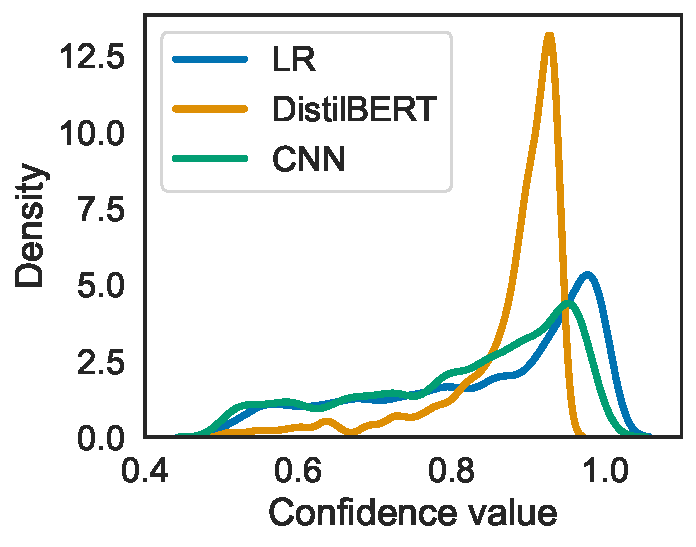
\includegraphics[scale=.40]{Figures/confidence-densities-seen-tp.pdf}
        \caption{TP}
    \end{subfigure}
    \begin{subfigure}{.35\textwidth}
        \centering
        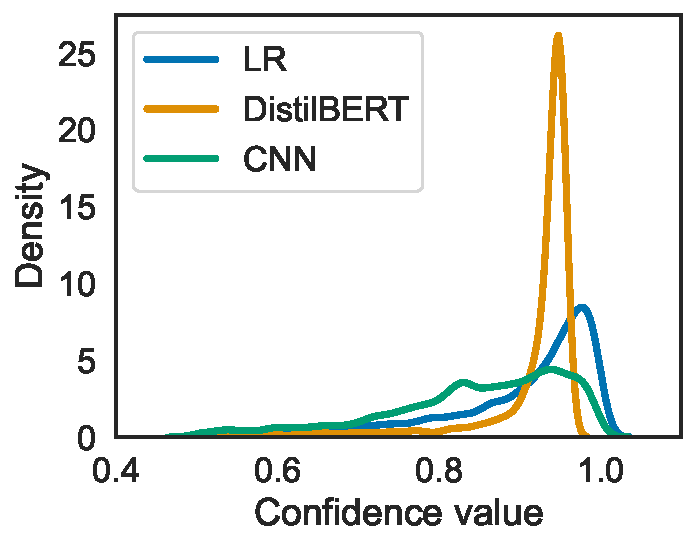
\includegraphics[scale=.40]{Figures/confidence-densities-seen-tn.pdf}
        \caption{TN}
    \end{subfigure}
    \begin{subfigure}{.35\textwidth}
        \centering
        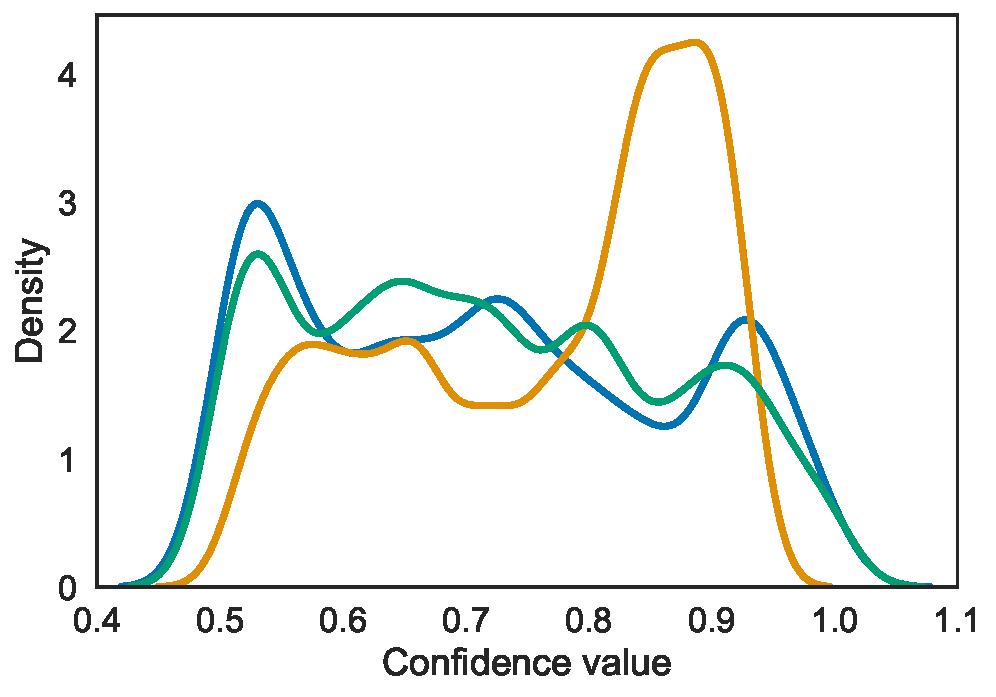
\includegraphics[scale=.40]{Figures/confidence-densities-seen-fp.pdf}
        \caption{FP}
    \end{subfigure}
    \begin{subfigure}{.35\textwidth}
        \centering
        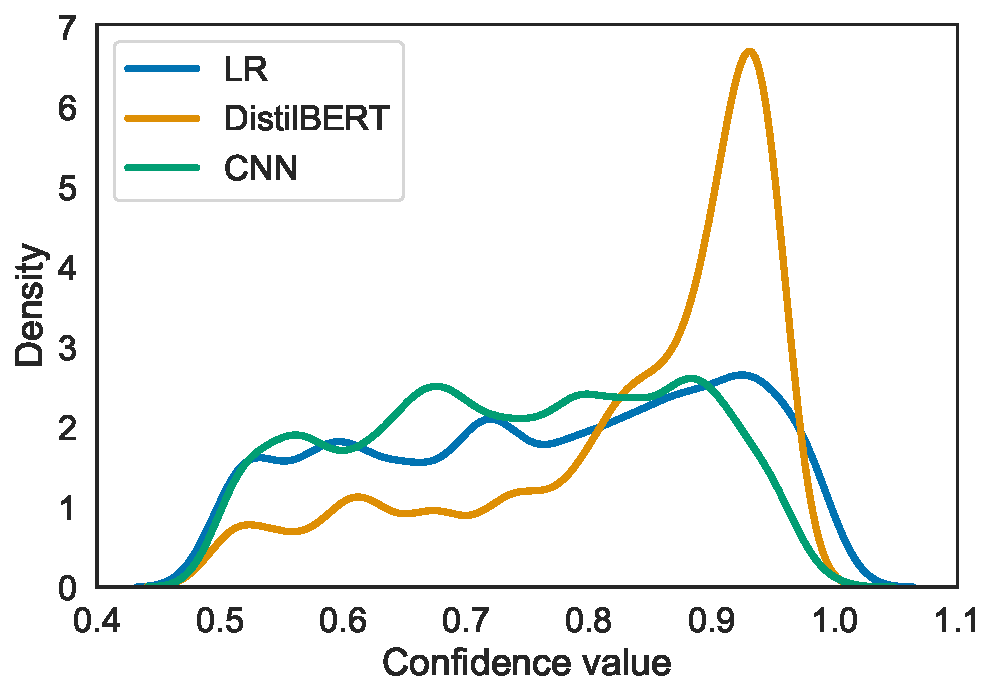
\includegraphics[scale=.40]{Figures/confidence-densities-seen-fn.pdf}
        \caption{FN}
    \end{subfigure}
    \caption{\textbf{Seen data}: Probability Density Functions of the confidence values of all predictions for the \emph{seen data} estimated with Kernel Density Estimation.}
    \label{fig:pdfs-seen}
\end{figure}

\begin{figure}[H]
    \centering
    \begin{subfigure}{.35\textwidth}
        \centering
        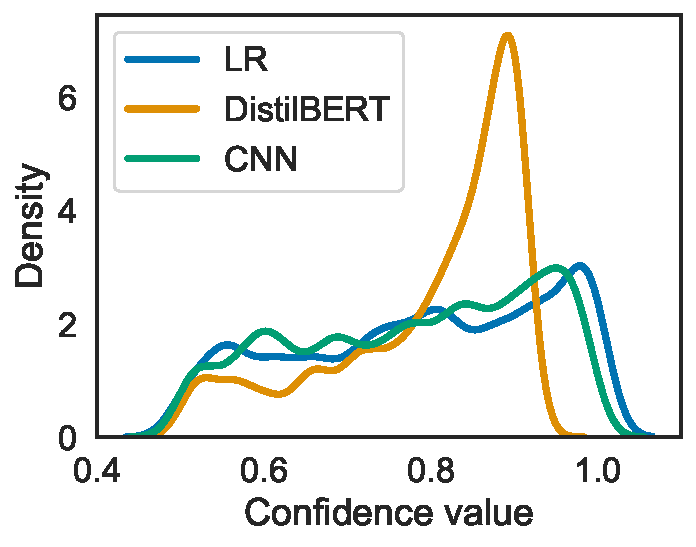
\includegraphics[scale=.40]{Figures/confidence-densities-unseen-tp.pdf}
        \caption{TP}
    \end{subfigure}
    \begin{subfigure}{.35\textwidth}
        \centering
        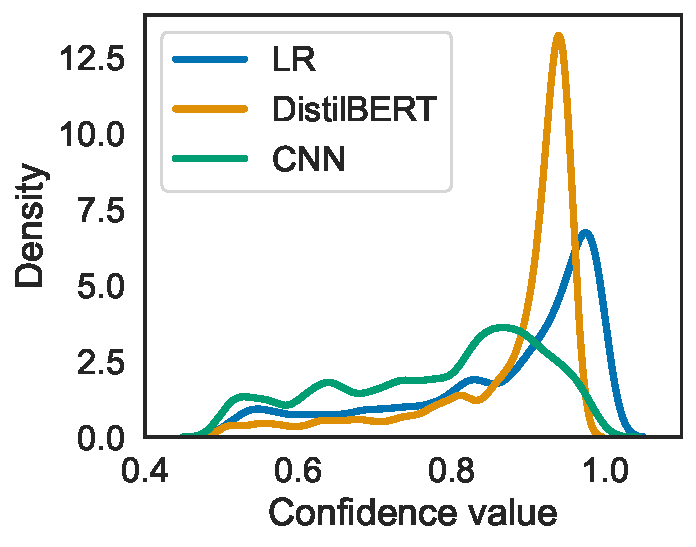
\includegraphics[scale=.40]{Figures/confidence-densities-unseen-tn.pdf}
        \caption{TN}
    \end{subfigure}
    \begin{subfigure}{.35\textwidth}
        \centering
        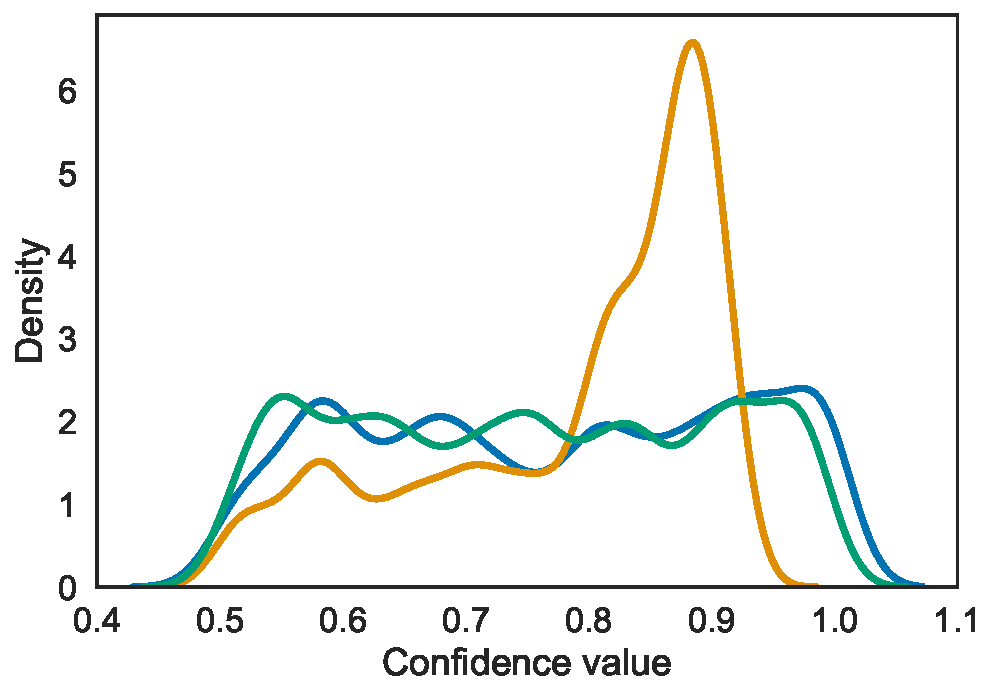
\includegraphics[scale=.40]{Figures/confidence-densities-unseen-fp.pdf}
        \caption{FP}
    \end{subfigure}
    \begin{subfigure}{.35\textwidth}
        \centering
        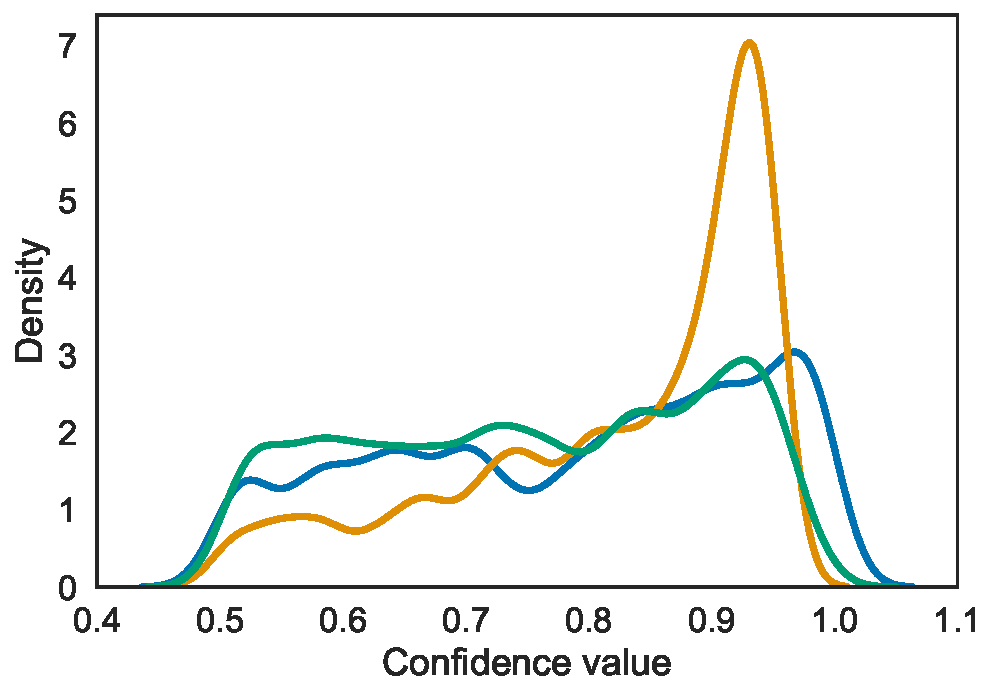
\includegraphics[scale=.40]{Figures/confidence-densities-unseen-fn.pdf}
        \caption{FN}
    \end{subfigure}
    \caption{\textbf{Unseen data}: Probability Density Functions of the confidence values of all predictions for the \emph{unseen data} estimated with Kernel Density Estimation.}
    \label{fig:pdfs-unseen}
\end{figure}